\newpage
\section{Test 6}
\label{Sec:test_6}

In the sixth test setting rover is dropped onto the horizontal plane.
A spherical obstacle has been set in front of the rover. The obstacle is in the form of a part of sphere which protudes outside the plane.
Center of the sphere has been set so that the protrusion is equal to $40$ $cm$.

\begin{figure}[H]
  \centering
    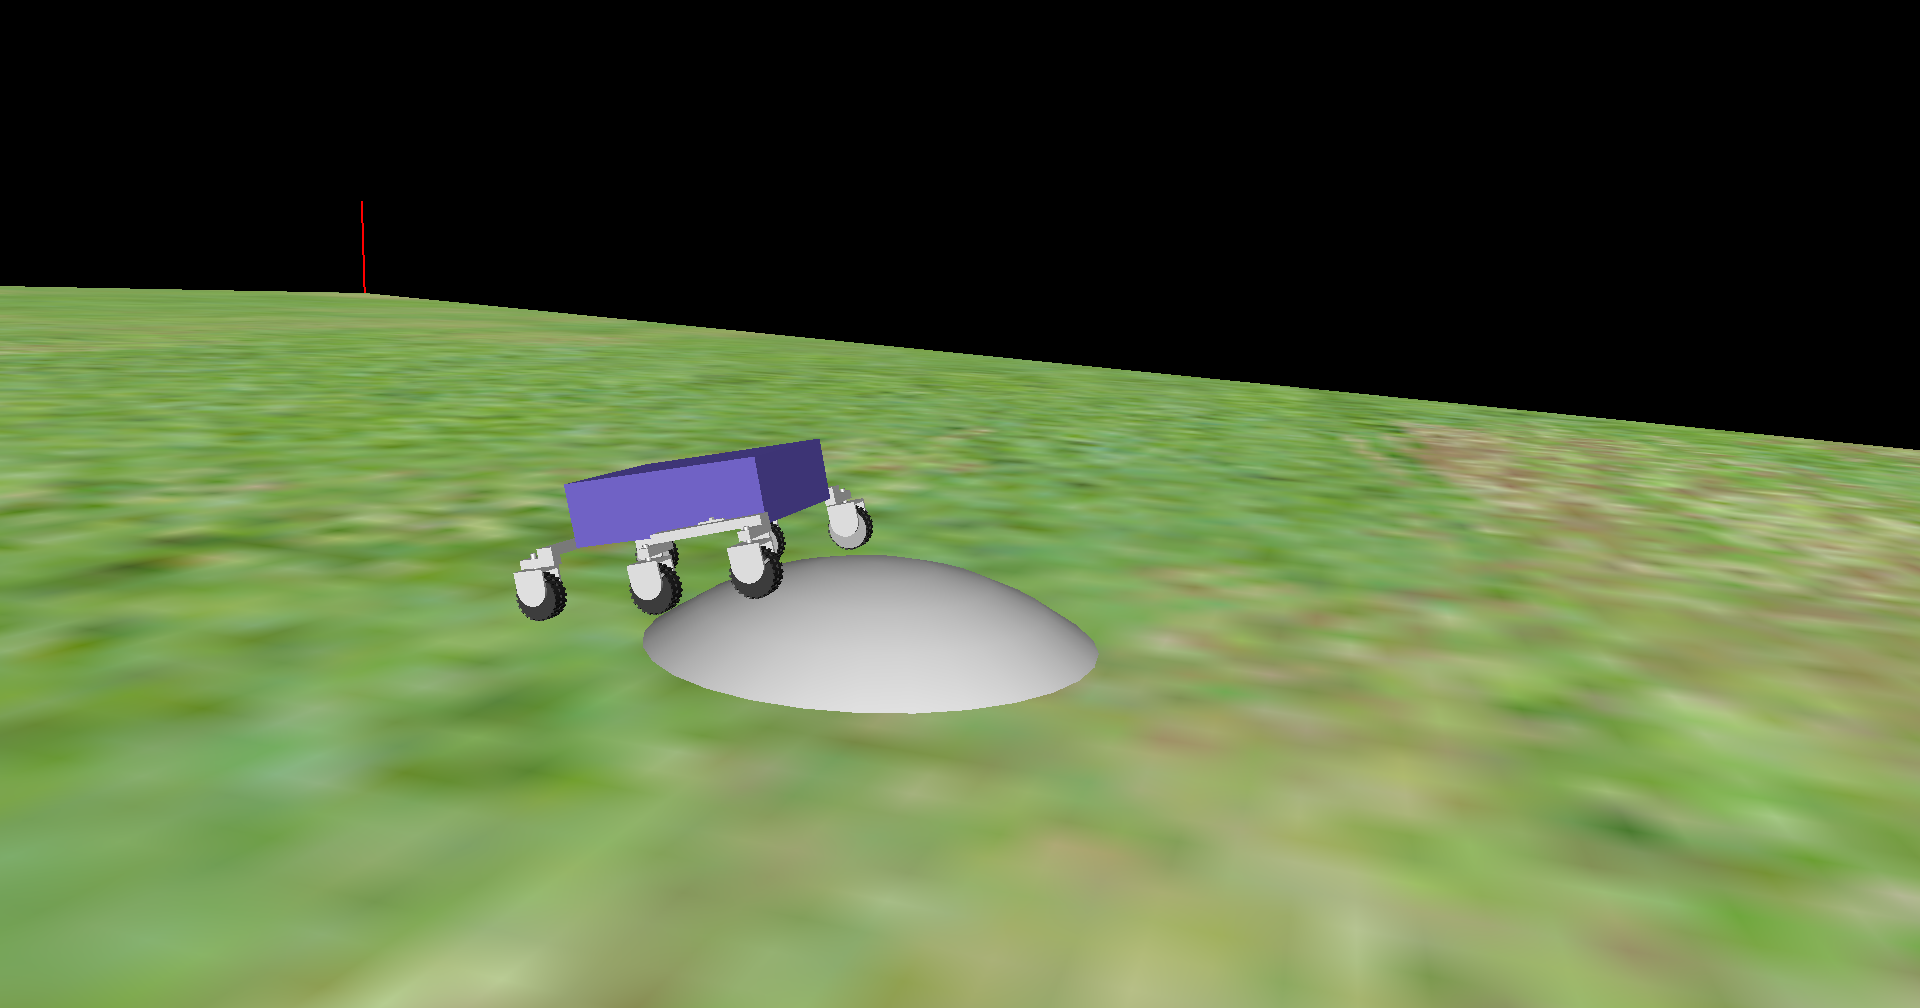
\includegraphics[width=0.8\textwidth]{run_6}
  \caption{Sixth test scenario}
\end{figure}

\noindent In this case, following quantities have been plotted:

\begin{itemize}
  \item $x_{COM}$ - mass center coordinates
\end{itemize}

\begin{figure}[H]
  \centering
    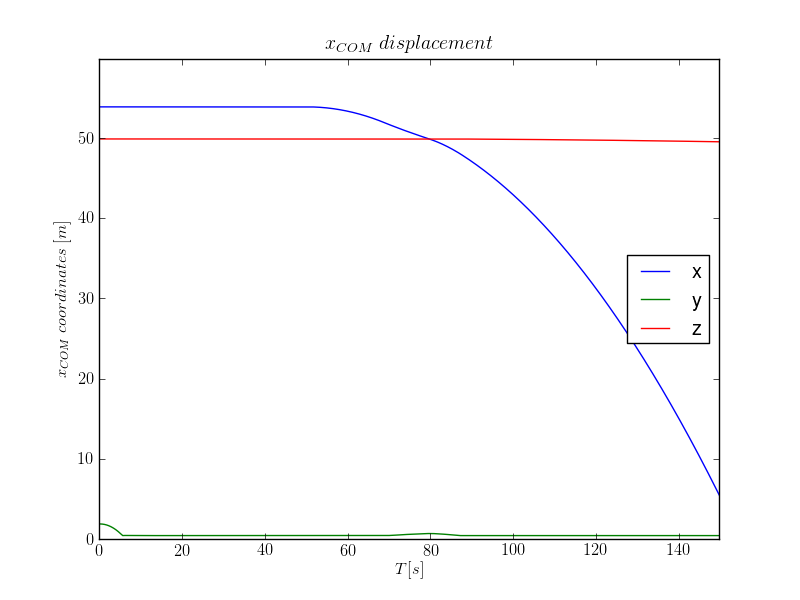
\includegraphics[width=0.8\textwidth]{xCOM6}
  \caption{$x_{COM}$}
\end{figure}

\begin{itemize}
  \item $x_{wheels}$ - wheels angular displacement 
\end{itemize}

\begin{figure}[H]
  \centering
    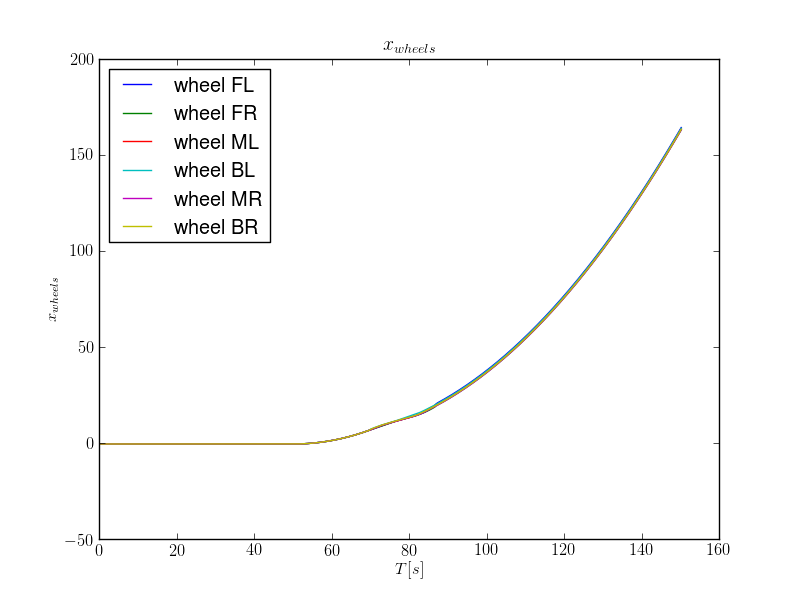
\includegraphics[width=0.8\textwidth]{xWHEELS6}
  \caption{$x_{wheels}$}
\end{figure}

\begin{itemize}
  \item $v_{COM}$ - mass center velocity
\end{itemize}

\begin{figure}[H]
  \centering
    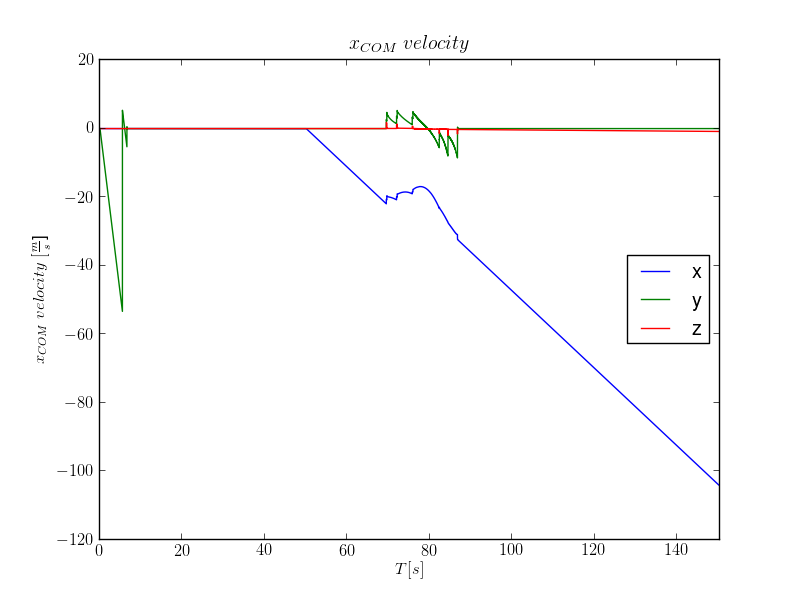
\includegraphics[width=0.8\textwidth]{vCOM6}
  \caption{$v_{COM}$}
\end{figure}

\begin{itemize}
  \item $v_{wheels}$ - wheels angular velocity
\end{itemize}

\begin{figure}[H]
  \centering
    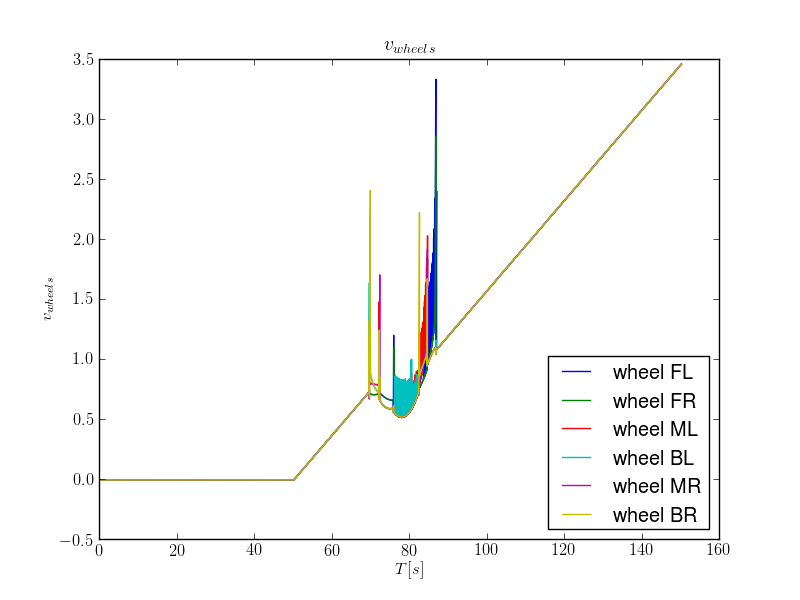
\includegraphics[width=0.8\textwidth]{vWHEELS6}
  \caption{$v_{wheels}$}
\end{figure}

\begin{itemize}
  \item $R_{COM}$ - reaction forces of center of mass in lagrangian coordinates
\end{itemize}

\begin{figure}[H]
  \centering
    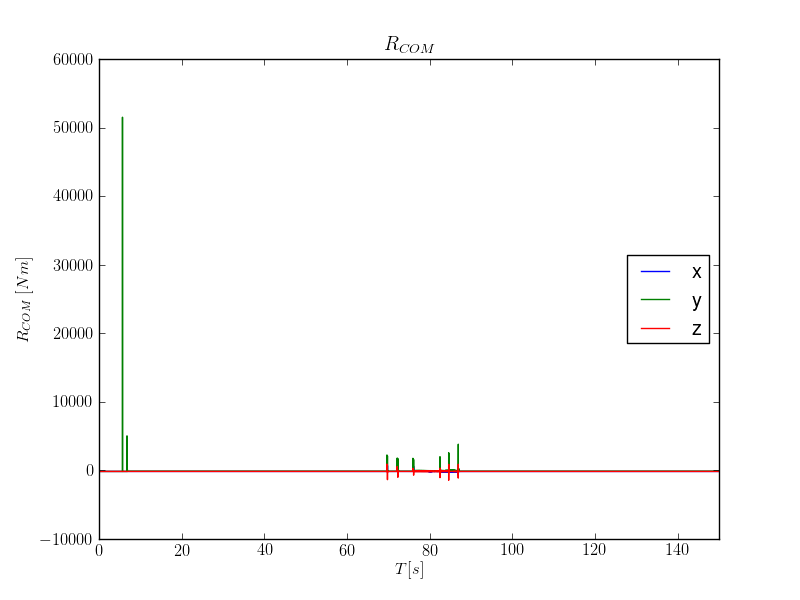
\includegraphics[width=0.8\textwidth]{pCOM6}
  \caption{$R_{COM}$}
\end{figure}

\begin{itemize}
  \item $R_{wheels}$ - reaction forces of wheels in lagrangian coordinates
\end{itemize}

\begin{figure}[H]
  \centering
    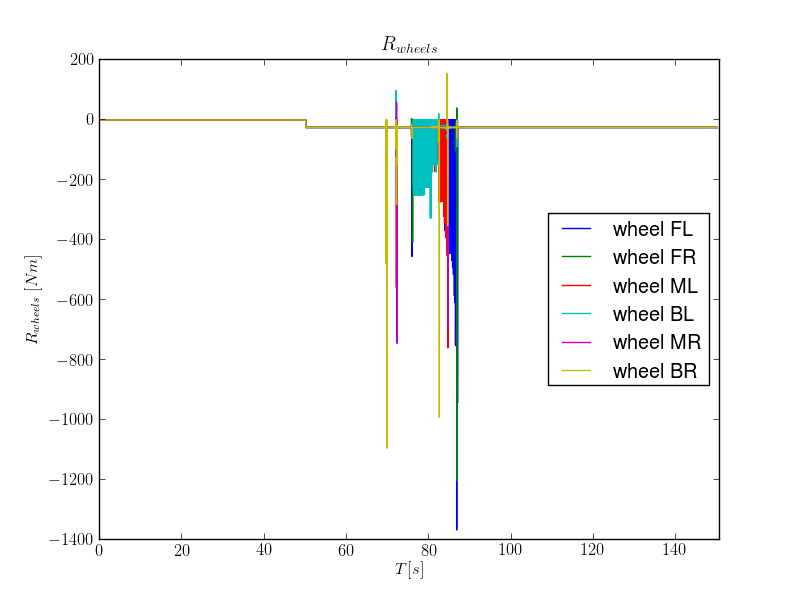
\includegraphics[width=0.8\textwidth]{pWHEELS6}
  \caption{$R_{wheels}$}
\end{figure}

\begin{itemize}
  \item $\lambda_{N}$ - normal component of the contact force (impulsion) for each wheel (interaction with the plane) zoomed when on the sphere
\end{itemize}

\begin{figure}[H]
  \centering
    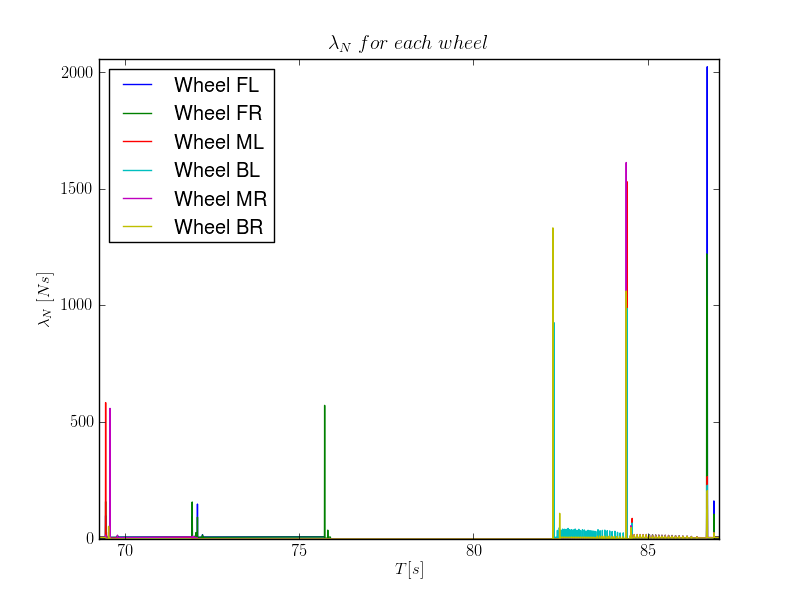
\includegraphics[width=0.8\textwidth]{lambdaN6}
  \caption{$\lambda_{N}$}
\end{figure}

\begin{itemize}
  \item $\lambda_{N}$ - normal component of the contact force (impulsion) for each wheel (interaction with the sphere) zoomed when on the sphere
\end{itemize}

\begin{figure}[H]
  \centering
    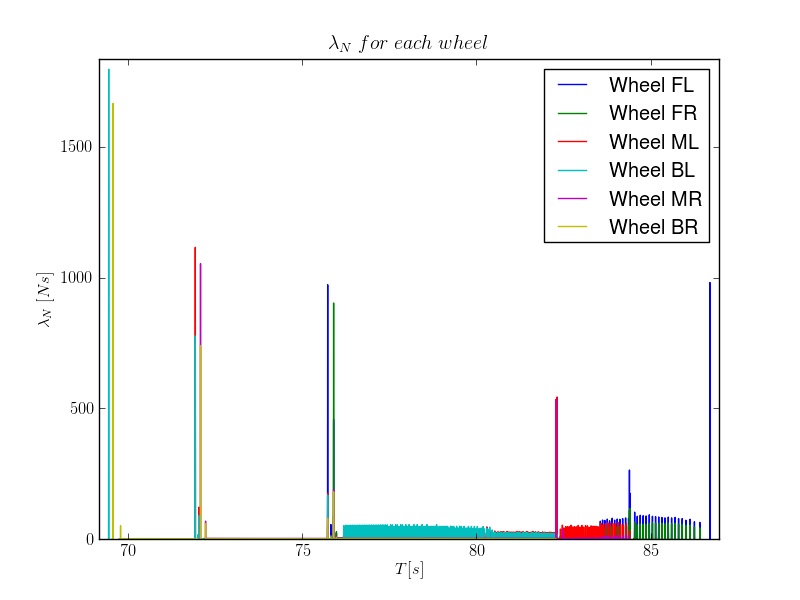
\includegraphics[width=0.8\textwidth]{lambdaN6sphere}
  \caption{$\lambda_{N}$}
\end{figure}

\begin{itemize}
  \item $\lambda_{T_x}$ - tangential component of the contact force in the x direction for each wheel
\end{itemize}

\begin{itemize}
  \item $\lambda_{T_z}$ - tangential component of the contact force in the z direction for each wheel
\end{itemize}

\begin{itemize}
  \item $y_{N}$ - gap function (distance between contact point and the constraint function) for each wheel (interaction with the plane) when on the sphere
\end{itemize}

\begin{figure}[H]
  \centering
    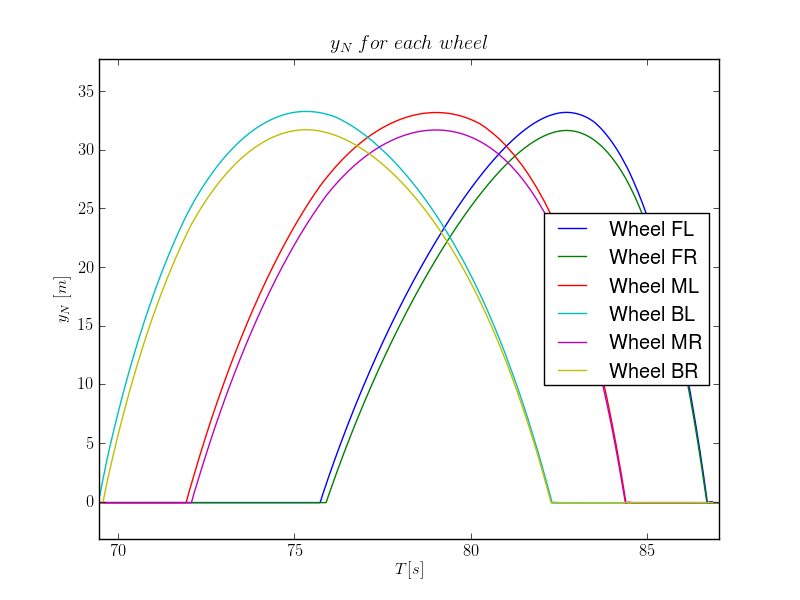
\includegraphics[width=0.8\textwidth]{yN6plane}
  \caption{$y_{N}$}
\end{figure}

\begin{itemize}
  \item $y_{N}$ - gap function (distance between contact point and the constraint function) for each wheel (interaction with the sphere) when on the sphere
\end{itemize}

\begin{figure}[H]
  \centering
    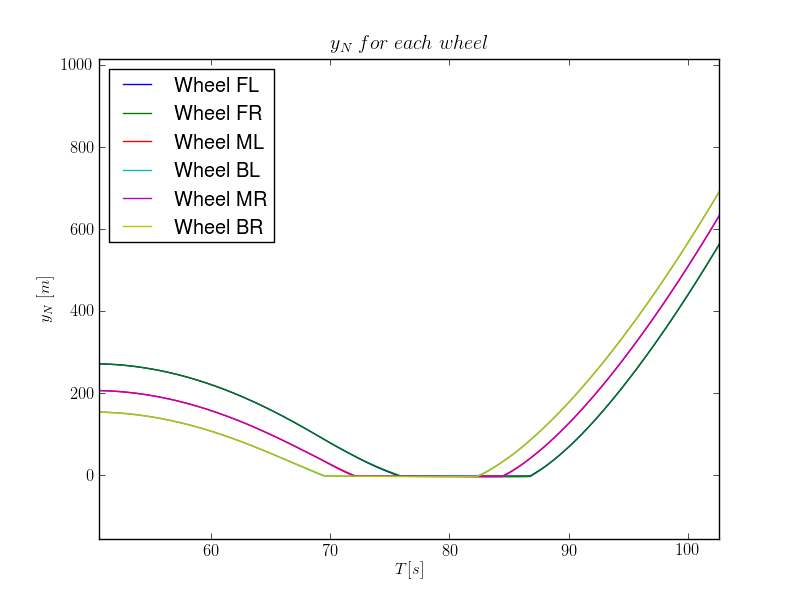
\includegraphics[width=0.8\textwidth]{yN6sphere}
  \caption{$y_{N}$}
\end{figure}







%\begin{itemize}
%  \item $\dot{y}_{N}$ - normal component of the local contact velocity for each wheel
%\end{itemize}
%
%\begin{itemize}
%  \item $\dot{y}_{T_x}$ - tangential component x of the local contact velocity for each wheel
%\end{itemize}
%
%\begin{itemize}
%  \item $\dot{y}_{T_z}$ - tangential component z of the local contact velocity for each wheel
%\end{itemize}


